\documentclass[11pt,twoside,a4paper]{article}

\usepackage[dutch]{babel}
\usepackage{a4wide} % Bladgroote is A4
\usepackage{enumitem}
\usepackage{graphicx} % Om figuren te kunnen verwerken
\usepackage{verbatim} 
\usepackage{parskip} % witruimte tussen paragrafen introduceren.
\usepackage[nottoc]{tocbibind}
\usepackage[normal]{caption}
\usepackage{hyperref}
%\usepackage[ampersand]{easylist}


\title{Performantie}

\newcommand{\logo}{../latex_extra/images/ugent.png}

\begin{document}

\newcommand{\HRule}{     % lijn tekenen ===> wordt gebruikt in titlepage
	\rule{\linewidth}{0.5mm}
}

\author{
	Tr\'esor Akimana\\
	Nick De Smedt\\
	Tom Hoet\\
	Dean Parmentier\\
	Simon Scheerlynck\\
	Xavier Seyssens\\
	Jonas Van Wilder\\
	Lennart Vermeir
}
\date{2015-2016}

\makeatletter		%zorgt ervoor dat we de macros kunnen gebruiken die met @ beginnen
\begin{titlepage}

		\center
		 
		\textsc{\LARGE Universiteit Gent}\\[1.5cm]
		\textsc{\Large Vakoverschrijdend project}\\[0.5cm]
		\textsc{\large Project Mobiliteitsbedrijf Gent}\\[0.5cm]

		\HRule \\[0.4cm]
		{ \huge \bfseries \@title }\\[0.4cm]
		\HRule \\[1.5cm]
		 
		\begin{minipage}{0.4\textwidth}
			\begin{flushleft} \large
				\emph{Groep 7:}\\
				\@author
			\end{flushleft}
		\end{minipage}
			~
		\begin{minipage}{0.4\textwidth}
			\begin{flushright} \large
				\emph{Lesverantwoordelijken:}\\
				Jan \textsc{Goedgebeur}\\
				Annick \textsc{Van Daele}\\
				Prof. Dr. Marko \textsc{Van Dooren}
			\end{flushright}
		\end{minipage}\\[4cm]


		{\large \@date}\\[1cm]


		\includegraphics[width=0.3\textwidth]{\logo}

\end{titlepage}
\makeatother %annuleren \makeatletter

\section*{Backend}
 
 Om de performantie van de applicatie live te monitoren op de server hebben we gebruik gemaakt van Java Melody. Deze bevindt zich ook in de jar van de applicatie en wordt dus tegelijk uitgevoerd. De resultaten van deze monitoring zijn beschikbaar op de webgui (https://vopro7.ugent.be/monitoring) en in pdf formaat (Git repository: documentation/milestone3/ op Master). De resultaten in de pdf zijn van een periode van circa 2 weken. Bij het analyseren van deze resultaten moet wel rekening worden gehouden, dat de monitoring niet gebeurde op een volledig systeem in gebruik, maar op een applicatie in ontwikkeling dat nog niet veel data bevatte. Vaak worden bepaalde gemiddelde uitvoeringstijden in het rood aangeduid door Java Melody. We moeten deze echter negeren omdat dit vaak berekend is op basis van één enkel request naar een url van een bepaalde user.
 \par Toch zien we hier al dat er een bottleneck is in de Postgres databank, namelijk bij de query die events en users met elkaar linkt, en dan vooral bij het verwijderen van de overbodige links uit de databank. (\textbf{DELETE FROM matchedEvents WHERE event\_id = ?}). Deze heeft een gemiddelde uitvoeringstijd van 1,5 seconden, wat ten opzichte van de totale tijd gespendeerd aan sql queries neerkomt dat ongeveer 97\% hieraan gespendeerd wordt. Dit komt omdat er extreem veel events gematcht moeten worden en dat deze vaak toegevoegd of verwijderd worden in de databank. We hebben geprobeerd om de query minder vaak uit te voeren door niet alle matches voor een event telkens te verwijderen, maar enkel diegene die niet meer van toepassing zijn voordat de nieuwe matches worden toegevoegd. Er zijn dus nog zeker verdere optimalisaties mogelijk aan de matching en processing van events.
 Daarnaast kunnen we uit deze resultaten ook afleiden dat vooral het opvragen van events het meeste tijd vraagt. We zien dat 80\% van de tijd uitgevoerd in de SpringControllers besteed is aan het opvragen van events.
 
 
 Verder hebben we ook performantietesten gedaan met behulp van JMeter. We simuleerden de situatie waarin meerdere gebruikers tegelijk een lijst van alle events opvragen. In de praktijk is deze exacte situatie wel niet mogelijk aangezien deze beperkt is tot de rollen operator en admin. Een gelijkaardige situatie kan wel bekomen worden, wanneer veel gebruikers tegelijk de voor hen relevante events opvragen. Ze kunnen nog altijd bijvoorbeeld een interessepunt aanmaken voor heel Gent, zodat ze dus alle actieve events kunnen opvragen. In zo een situatie zou het bijvoorbeeld kunnen voorvallen dat 2000 gebruikers in een tijdspanne van 10 seconden hun events opvragen (circa 80). Het resultaat wordt weergegeven in onderstaande figuur.
 

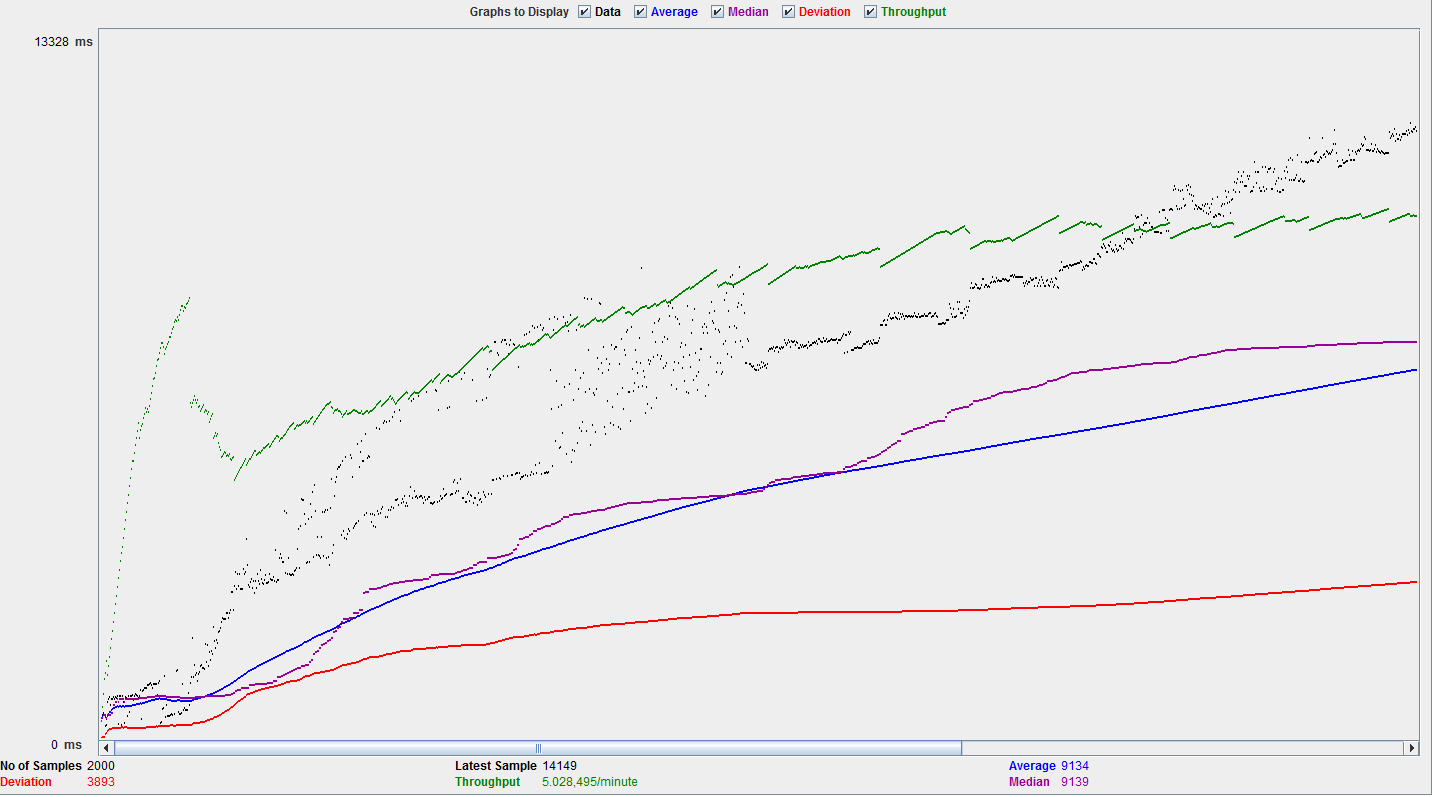
\includegraphics[scale=0.80, angle=90]{../latex_extra/images/graph.png}

\end{document}
